%\documentclass[nocopyrightspace]{sigplanconf}
%\documentclass{entcs} 
%\usepackage{entcsmacro}
\documentclass{article}
\usepackage{graphicx}
\usepackage{code,amsmath,math-cmds,url,alltt,verbatim}

\setlength{\oddsidemargin}{.22in}
\setlength{\evensidemargin}{.22in}
\setlength{\textwidth}{6.5in}


%\newcommand{\url}[1]{{\ensuremath{\mathtt {#1}}and}}

\begin{document}

\newcommand{\cut}[1]{}

\newcommand{\appref}[1]{Appendix~\ref{#1}}
\newcommand{\secref}[1]{Section~\ref{#1}}
\newcommand{\tblref}[1]{Table~\ref{#1}}
\newcommand{\figref}[1]{Figure~\ref{#1}}
\newcommand{\listingref}[1]{Listing~\ref{#1}}
%\newcommand{\pref}[1]{{page~\pageref{#1}}}

\newcommand{\eg}{{\em e.g.}}
\newcommand{\cf}{{\em cf.}}
\newcommand{\ie}{{\em i.e.}}
\newcommand{\etc}{{\em etc.\/}}
\newcommand{\naive}{na\"{\i}ve}
\newcommand{\role}{r\^{o}le}
\newcommand{\forte}{{fort\'{e}\/}}
\newcommand{\appr}{\~{}}

\newcommand{\bftt}[1]{{\ttfamily\bfseries{}#1}}
\newcommand{\kw}[1]{\bftt {#1}}
\newcommand{\Pthen}{\kw{Pthen}}
\newcommand{\pads}{\textsc{pads}}
\newcommand{\padsl}{\textsc{padsl}}
\newcommand{\padst}{\textsc{pads/t}}
\newcommand{\datatype}{\textsc{PADS/T}}
%\newcommand{\datatype}{\textsc{DataType}}
\newcommand{\C}{\textsc{C}}
\newcommand{\perl}{\textsc{Perl}}
\newcommand{\ml}{\textsc{ml}}
\newcommand{\sml}{\textsc{sml}}
\newcommand{\smlnj}{\textsc{sml/nj}}
\newcommand{\java}{\textsc{java}}
\newcommand{\ddl}{\textsc{ddl}}
\newcommand{\xml}{\textsc{xml}}
\newcommand{\datascript}{\textsc{DataScript}}
\newcommand{\packettypes}{\textsc{PacketTypes}}
\newcommand{\erlang}{\textsc{Erlang}}

\newcommand{\Core}{Ad hoc}
\newcommand{\core}{ad hoc}
\newcommand{\pvalue}{\core{} value}
\newcommand{\ppat}{\core{} pattern}
\newcommand{\ptype}{\core{} type}

\newcommand{\padsc}{\textsc{pads}/\C{}}
\newcommand{\padsml}{\textsc{pads}/\ml{}}

\newcommand{\dibbler}{Sirius}
\newcommand{\ningaui}{Altair}
\newcommand{\darkstar}{Regulus}

\newcommand{\pdgood}{{\tt G}}
\newcommand{\pdbad}{{\tt B}}
\newcommand{\pdnest}{{\tt N}}
\newcommand{\pdsem}{{\tt S}}
\newcommand{\ptypes}{T}
\newcommand{\patreadpd}[2]{{\tt #1<<#2>>}}
\newcommand{\btm}{\cd{BOT}}


\newcommand{\lsem}{{[\![}}
\newcommand{\rsem}{{]\!]}}


\newcommand{\figHeight}[4]{\begin{figure}[tb]
	\centerline{
	            \epsfig{file=#1,height=#4}}
	\caption{#2}
	\label{#3}
	\end{figure}}

%% Environment for typesetting BNF grammars. Uses display math mode.
\newenvironment{bnf}
     {%% local command definitions:
        %% BNF definition symbol
      \def\->{\rightarrow}
%%      \def\::={{::=} &}
      \def\::={\bnfdef &}
      \def\|{\bnfalt}
      \newcommand{\name}[1]{\text{##1}}
        %% non-terminal
      \newcommand{\nont}[1]{{##1}}
      \newcommand{\meta}[1]{& ##1 &}
      \newcommand{\descr}[1]{& \text{// ##1}}
      \newcommand{\opt}[1]{ [##1] }
      \newcommand{\opnon}[1]{\opt{\nont{##1}}}
      \newcommand{\none}{\epsilon}
      \newcommand{\nwln}{\\ &&&}
      \newcommand{\nlalt}{\\ && \| &}
      \[\begin{array}{lrlll}
     }
     {\end{array}\]}

\newcommand{\mcd}[1]{\mathtt{#1}}
\newcommand{\ppair}[3]{#1{:}#2 \mathrel{**} #3}
\newcommand{\parray}[3]{#1\;\mcd{Parray}(#2,#3)}
\newcommand{\pset}[3]{\{#1{:}#2\,|\,#3\}}
\newcommand{\pstream}[1]{#1\;\mcd{stream}}
\newcommand{\precord}[1]{\{\{#1\}\}}



% A couple of exemplary definitions:
%\def\lastname{Fernandez, Fisher, Mandelbaum and Walker}



%\begin{frontmatter}

  \title{\datatype{}: \\ A Language for Describing and Transforming Ad Hoc Data} 

%  \authorinfo{
\author{Mary Fernandez and
     Kathleen Fisher, AT\&T Research\\ 
    Yitzhak Mandelbaum and  David Walker, Princeton University}
%\thanksref{attemail}}
%   \address{AT\&T\\ 
%     Florham Park,NJ USA} 
%   \authorinfo{Yitzhak Mandelbaum,
%     David Walker\thanksref{premail}}
%    \address{Department of Computer Science\\ 
%      Princeton University\\
%      Princeton,NJ USA} 
%    \thanks[attemail]{Email:\texttt{\normalshape
%          mff,kfisher@research.att.com}}
%    \thanks[premail]{Email:\texttt{\normalshape
%          yitzhakm,dpw {\it at} cs {\it dot} princeton {\it dot} edu}}


\maketitle

\begin{abstract}
\datatype{} is a declarative data description language paired with an 
error-aware transformation language.  This pairing provides rich support for
programming with ad hoc data sources.  Such data is common in a wide range of domains including networking, financial analysis, biology, and physics.
\datatype{}'s data description language is based on polymorphic, recursive, and dependent data types.  From such descriptions, the compiler generates robust parsing and pretty printing code. The transformation language supports \textit{error-aware computation} by automatically maintaining an association between data and a description of the errors in that data.  
\end{abstract}

% \begin{keyword}
% Ad hoc data, semi-structured data, data description, data transformation, pattern matching, dependent types.
% \end{keyword}
% \end{frontmatter}

\section{Introduction}
\label{sec:intro}

{\em Data description languages} are a class of domain specific
languages for specifying {\em ad hoc data formats}, from billing 
records to TCP packets to scientific data sets to server logs.  Examples 
of such languages include 
\bro~\cite{paxson:bro}, \datascript{}~\cite{gpce02}, \demeter~\cite{lieberherr+:class-dictionaries},
\packettypes{}~\cite{sigcomm00}, \padsc{}~\cite{fisher+:pads}, 
\padsml{}~\cite{mandelbaum+:padsml}  and
\xsugar~\cite{xsugar2005}, among others.  All of these languages
generate parsers from data descriptions.  In addition, and unlike
conventional parsing tools such as Lex and Yacc, many also automatically
generate auxiliary tools ranging from printers to \xml{} converters to
visitor libraries to visualization and editor tools.

In previous work, we developed the {\em Data Description Calculus}
(\ddcold{}), a calculus of simple, orthogonal type constructors,
designed to capture the core features of many existing type-based data
description languages~\cite{fisher+:next700ddl,fisher+:ddcjournal}.
This calculus had a multi-part denotational semantics that interpreted
the type constructors as (1) parsers the transform external bit
strings into internal data representations and {\em parse descriptors}
(representations of parser errors), (2) types for the data
representations and parse descriptors, and (3) types for the parsers
as a whole.  We proved that this multi-part semantics was coherent in
the sense that the generated parsers always have the expected types
and generate representations that satisfy an important {\em
canonical forms} lemma.

The \ddcold{} has been very useful already, helping us debug and
improve several aspects of \padsc{}~\cite{fisher+:pads}, and serving
as a guide for the design of \padsml{}~\cite{mandelbaum+:padsml}.
However, this initial work on the \ddcold{} told only a fraction of the
semantic story concerning data description languages.  As mentioned
above, many of these languages not only provide parsers, but
also other tools.  Amongst the most common auxiliary tools
are printers, as reliable communication between programs, either through
the file system or over the Web, depends upon both input (parsing) 
and output (printing).

In this work, we begin to address the limitations of
\ddcold{} by specifying a printing semantics for the
various features of the calculus.  We also
prove a collection of theorems for the new semantics that serve as
duals to our theorems concerning parsing.  This new printing semantics
has many of the same practical benefits as our older parsing 
semantics: We can
use it as a check against the correctness of our printer
implementations and as a guide for the
implementation of future data description languages.  


% First, we extend \ddcold{} with
% abstractions over types, which provides a basis for specifying the
% semantics of \padsml{}. In the process, we also improve upon the
% \ddcold{} theory by making a couple of subtle changes. For example, we
% are able to eliminate the complicated ``contractiveness'' constraint
% from our earlier work. Second, .

% The main practical benefit of the calculus has been as a guide for our
% implementation. Before working through the formal semantics, we
% struggled to disentangle the invariants related to polymorphism. After
% we had defined the calculus, we were able to implement type
% abstractions as \ocaml{} functors in approximately a week.  Our new
% printing semantics was also very important for helping us define and
% check the correctness of our printer implementation.  We hope the
% calculus will serve as a guide for implementations of \pads{} in
% other host languages.  

% In summary, this work makes the following key contributions:
% \begin{itemize}
% \item We simultaneously specify both a parsing and a printing semantics
%   for the \ddc{}, a calculus of polymorphic, dependent types.
% \item We prove that \ddc{} parsers and printers are type safe
%   and well-behaved as defined by a canonical forms theorem.
% \end{itemize}

In this extended abstract, we give an brief overview of the calculus,
it's dual semantics and their properties.  A companion technical
report contains a complete formal
specification~\cite{fisher+:popl-sub-long}.  In comparison to our
previous work on the \ddcold{} at POPL 06~\cite{mandelbaum+:padsml},
the calculus we present here has been streamlined in several subtle,
but useful ways.  It has also been improved through the addition of
polymorphic types.  We call this new polymorphic variant
\ddc{}.  These improvements and extensions, together with
proofs, appear in Mandelbaum's thesis~\cite{mandelbaum:thesis} and in
a recently submitted journal article~\cite{fisher+:ddcjournal}.
This abstract reviews the \ddc{} and extends all the previous 
work with a printing semantics and appropriate theorems.
To be more specific,
sections~\ref{sec:ddc-syntax} through \ref{sec:ddc-sem} present the
extended \ddc{} calculus, focusing on the semantics of polymorphic
types for parsing and the key elements of the printing semantics.
Then, \secref{sec:meta-theory} shows that both parsers and
printers in the \ddc{} are type correct and furthermore that parsers
produce pairs of parsed data and parse descriptors in {\em canonical
  form}, and that printers, given data in canonical form, print
successfully. We briefly discuss related work in \secref{sec:related}, and
conclude in \secref{sec:conc}.

%%% Local Variables: 
%%% mode: latex
%%% TeX-master: "paper"
%%% End: 


\section{Describing Data in \datatype{}}
\label{sec:data-description}

A \datatype{} description specifies the physical layout and semantic
properties of an ad hoc data source.  
These descriptions are composed of types: 
base types describe atomic data, while structured
types describe compound data built from simpler pieces.  Examples of
base types include 8-bit unsigned integers (\cd{Puint8}), 32-bit
integers (\cd{Pint32}), binary 32-bit integers (\cd{Pbint32}), dates
(\cd{Pdate}), strings (\cd{Pstring}), and IP addresses (\cd{Pip}).
Semantic conditions for such base types include checking that the
resulting number fits in the indicated space, \ie, 16-bits for
\cd{Pint16}.

Base types (and other types) may be parameterized by values.  This
mechanism serves both to reduce the number of base types and to permit
the format and properties of later portions of the data to depend upon
earlier portions.  For example, the base type \cd{Puint16_FW(3)}
specifies an unsigned two byte integer physically represented by
exactly three characters. The base type \cd{Pstring} takes 
a string indicating the set of acceptable terminator characters. Hence, 
\cd{Pstring(";|")} can be terminated by either a semicolon or a
vertical bar.


To describe more complex data, \datatype{} provides a collection of
type constructors derived from the type structure of functional
programming languages such as Haskell and ML.  The following
subsections will explain these structured types through a series 
of real-world examples.  Readers eager to see the complete syntax
of types should flip forward to Appendix~\ref{app:syntax-dd}.

\subsection{Simple Structured Descriptions}

The bread and butter of any \datatype{} description are the
simple structured types: tuple, record and array types for expressing
sequences of data; sum types, realized here as datatypes, for
expressing alternatives; and singleton types for expressing
the placement of particular character in data.  In this section, we
explain each of these items by building a description 
of the \dibbler{} data presented in \figref{figure:dibblerml}.

The \dibbler{} data source is used to record summaries of
phone orders produced at AT\&T.  Each summary
involves a date and one record per order.
Each order record contains a header followed by a sequence of events.
The header has 13 pipe separated fields: the order number, AT\&T's
internal order number, the order version, four different telephone
numbers associated with the order, the zip code of the order, a
billing identifier, the order type, a measure of the complexity of the
order, an unused field, and the source of the order data.  Many of
these fields are optional, in which case nothing appears between the
pipe characters.  The billing identifier may not be available at the
time of processing, in which case the system generates a unique
identifier, and prefixes this value with the string ``no\_ii'' to
indicate the number was generated. The event sequence represents the
various states a service order goes through; it is represented as a
new-line terminated, pipe separated list of state, timestamp pairs.
There are over 400 distinct states that an order may go through during
provisioning.  The sequence is sorted in order of increasing timestamps. 
%\figref{figure:dibbler-records} shows a small example of
%this format.
%156 different states for one order
%-rw-r--r--    1 angusm   dibbler   2187472314 Jun  9  2003 /fs/dibblerd/tlf/data/out_sum.stream
%2171.364u 31.379s 40:41.54 90.2% 0+0k 2+0io 2pf+0w
%53 had trailing t or } after zip code
%It may be apparent from this paragraph that English is a poor
%language for describing data formats!


\begin{figure*}
\begin{small}
%\begin{center}
\begin{verbatim}
0|1005022800
9152|9152|1|9735551212|0||9085551212|07988|no_ii152272|EDTF_6|0|APRL1|DUO|
9153|9153|1|0|0|0|0||152268|LOC_6|0|FRDW1|DUO|
\end{verbatim}
\caption{Miniscule example of \dibbler{} data.}
\label{figure:dibbler-records}
%\end{center}
\end{small}
\end{figure*}

\suppressfloats

\begin{figure}
\begin{code}
\kw{type} summary\_header = <"0|"> * Puint32 * <NL>
\mbox{}
\kw{datatype} dib\_ramp = 
  Ramp of Puint64 
| GenRamp of <"no\_ii"> * Puint64
\mbox{}
\kw{type} order\_header = \{
       order\_num      : Puint32;
 '|';  att\_order\_num  : Puint32;             
 '|';  ord\_version    : Puint32;         
 '|';  service\_tn     : pn\_t \kw{Popt};
 '|';  billing\_tn     : pn\_t \kw{Popt};          
 '|';  nlp\_service\_tn : pn\_t \kw{Popt};
 '|';  nlp\_billing\_tn : pn\_t \kw{Popt};
 '|';  zip\_code       : Pzip \kw{Popt};
 '|';  ramp           : dib\_ramp; 
 '|';  order\_sort     : Pstring('|');
 '|';  order\_details  : Puint32;             
 '|';  unused         : Pstring('|');
 '|';  Pstring('|')   : stream;
 '|';
\}
\mbox{}
\kw{type} event  = Pstring('|') *  <'|'> * Puint32
\mbox{}
\kw{type} events = event Parray('|',NL)
\mbox{}
\kw{type} source = summary\_header * (order\_header * events) Parray(NL,EOF)
\end{code}
\caption{\datatype{} description for \dibbler{} provisioning data.}
\label{figure:dibblerml}
\end{figure}


\figref{figure:dibblerml} gives a \datatype{} description for the
\dibbler{} phone order summaries in our syntax.  Overall, the description 
is a sequence of type definitions.  It is probably
easiest to understand the data source by reading these definitions
bottom up.

The last type definition \cd{source} is intended to be a definition of
an entire \dibbler{} data source.  It states that a
\cd{source} is a \cd{summery\_ header} followed by a sequence of
objects made up of an \cd{order\_header} followed by \cd{events}.  The
tuple type constructor (\cd{T1 ** T2}) and the array type constructor
(\cd{T Parray(sep,term)}) both specify sequences of objects in a data
source.  The \cd{Parray} type depends upon two value parameters,
(\cd{sep} and \cd{term}).  The first parameter describes the syntactic
separators that may be found between elements of the array.  In this
case \cd{Peor}, the {\em end-of-record} character, may be found 
between each element
of the array.  In this case, the end-of-record character 
should be set to a newline character as there is one record per
line in the file.   
The second parameter is the
terminator for the array.  In this case, the terminator is \cd{Peof}, the
end-of-file marker.  It is often necessary to have additional
termination conditions for arrays, such as termination dependent on
the number of elements read so far, but we omitted this additional option 
for expository purposes.

The definition of \cd{events} indicates that this part of the
\dibbler{} data will contain a sequence of \cd{event}s separated by
verticle bars and terminated by an end-of-record character.  
Each \cd{event} is a
string terminated by a veriticle bar, followed by a verticle bar and
ending with an unsigned 32-bit integer.  The interesting part of this
sequence is the presence of the type \cd{'|'}.  In type-theoretic
terms, this is a {\em singleton type}.  It states that one should
expect exactly the character \cd{'|'} in the input stream at this
point.  Other singletons appear in the summary header type as
\cd{"0|"} and \cd{Peor}.  Any expression that appears embedded in a type
as a singleton must be effect-free.

The type \cd{order\_header} is a record type that indicates
the data format involves the sequence of items described by
the fields of the record.  Notice that there are two different
sorts of fields: anonymous fields (a second form of singleton type) 
containing directives to parse a particular character (\cd{'|'}) or
string (\cd{"0|"})
and fields with names.  
% The second named field,
% \cd{att\_order\_num}, reveals two other proposed features of 
% \datatype: dependency and constraints.  Here,
% \cd{att\_order\_num} is constrained to be less than
% \cd{order\_num}, the value parsed in an earlier field.
% This is a relatively simple constraint on the correctness of the
% ad hoc data format.  In practice, constraints can become very rich
% involving properties such as sortedness of records in an array,
% definitions of expected characters,
% restrictions on date and time ranges, constraints on IP address
% domains, restrictions on phone number area codes and virtually 
% infinite variety of other possibilities. 

The last interesting feature in the \dibbler{} example is the
datatype definition of \cd{dib\_ramp}.  It describes
two alternatives for a portion of data, either an integer alone
or the fixed string \cd{"no\_ii"} followed by an integer.
In order to parse data in this format, the parser will
first attempt to parse the first branch and only if it
fails will it attempt to parse the second branch.
Notice how this semantics differs from similar constructs in
regular expressions and context-free grammars, which
non-deterministically choose between alternatives.
By making alternatives deterministic, we avoid
the need to implement general backtracking search.  
Fortunately, we have yet to come across an ad hoc data source
where we wish we had nondeterminisc choice.\footnote{\pads{}
can recognize string data based on regular expressions.
Non-determinism here has been useful, but as it
has been confined to parsing elements of the \cd{Pstring} 
base type, it has had no impact on the overall parsing 
algorithm.}

\begin{figure}
\begin{code}
val COMMA  = ','
val COLON  = ':'
val SEMI   = ';'
val LPAREN = '('
val RPAREN = ')'
\mbox{}
type entry = Pstring(COLON) ** COLON ** Pfloat32
\mbox{}
datatype tree =
    Tree of LPAREN ** tree Parray(COMMA,RPAREN) ** "):" ** Puint32
  | Tip of entry
\mbox{}
type source = (tree ** SEMI) Parray(NL,EOF)
\mbox{}
{\rm Tiny fragment of Newick data:} 
\mbox{}
(((erHomoC:0.28006,erCaelC:0.22089):0.40998,(erHomoA:0.32304,
(erpCaelC:0.58815,((erHomoB:0.5807,erCaelB:0.23569):0.03586,
erCaelA:0.38272):0.06516):0.03492):0.14265):0.63594,(TRXHomo:0.65866,
TRXSacch:0.38791):0.32147,TRXEcoli:0.57336);
\end{code}
\caption{Simplified tree-shaped Newick data}
\label{fig:newick}
\end{figure}

\subsection{Recursive Descriptions}

The original \pads{} design contained analogues of all the 
simple type constructors described in the previous section.
Hence, although the syntax of types we just saw
is more compact and more elegant than the C-style syntax 
of \pads, we have yet to add any expressive power. 
The first real step forward for \datatype{} is the introduction
of recursion through the data type mechanism.  While
recursion never appeared in the telecommunications and 
networking data sources \pads{} was initially designed for, it
appears essential for describing a number of biological
data sources we have encountered.
  
A representative example of such data comes courtesy of Steven
Kleinstein, program coordinator of Princeton's Picasso project for
interdisciplinary research in computational sciences.  Kleinstein is
in the process of building a simulator to study the
proliferation of B lymphocytes during an immune response.  Data
needed for his simulations is represented in a variant of the
Newick format, which is a flat
representation of trees and used by 
many biologists~\cite{newick}.  In Newick, 
leaves of the tree are string labels followed by a colon and a number.
A parent node in the tree introduces a collection of children by
placing a sequence of trees within parens.  Following the parens is a
colon and a number, as is the case for the leaf node.
The numbers represent the ``distance'' 
that separates the child from the parent.  In
Kleinstein's case, the distance is the number of mutations that occur
in the antibody receptor genes of B lymphocytes.   Each line
of a file may contain a different tree, terminated by a semi-colon.

\figref{fig:newick} gives a description of Newick and a short fragment 
of example data.  Despite the relative complexity of the structure of the data,
the description is remarkably concise and elegant.  Notice that the data type
definition of \cd{tree} is recursive --- we have not been able to find any
effective description of this data source without it.

\begin{figure}
  \centering
  \small
\begin{verbatim}
 2:3004092508||5001|dns1=abc.com;dns2=xyz.com|c=slow link;w=lost packets
 |INTERNATIONAL
 3:|3004097201|5074|dns1=bob.com;dns2=alice.com|src_addr=192.168.0.10;
 dst_addr=192.168.23.10;start_time=1234567890;end_time=1234568000;
 cycle_time=17412|SPECIAL
\end{verbatim}  
  \caption{Simplified network monitoring data.  This 
data containts two alarm records.  Extra newlines 
were inserted mid-record so the data would fit on a page.}
  \label{fig:darkstar-records}
\end{figure}

\subsection{Parameterized Descriptions}

The last key feature of \datatype{} is the ability to define
parameterized descriptions.  In \pads, description parameters
were limited to values.  In \datatype, descriptions
maybe parameterized by both values and types.  Type parameterization
introduces allows descriptions to be
reused at a variety of different types.  This feature 
helps make data descriptions
more concise and allows programmers to define convenient libraries
of reusable description components.

Our final example, shown in
Figure~\ref{fig:darkstar-records}, will illustrate 
the usefulness of descriptions parameterized by
both types and values and introduce a couple of other
useful features as well.   This example displays
alarm data recorded by a network link monitor
and used \darkstar{} project at AT\&T.  Each alarm signals some
problem with a network link.  

Now, at this point, we could write out an English description
of the \darkstar{} data, and indeed, in an earlier version of this paper
we did so.  However, English is a terrible specification language
for ad hoc data, and every description we have attempted to give has not 
only been imprecise, it has also made for some very 
boring reading.  Hence, we dispense with the informal
English and head straight for for the \datatype{} description,
which is shown in \figref{fig:darkstar-ml}.

% In our example,
% there are two classes of alarms, indicated with the integers 2 and 3.
% The alarm class is specified first, followed by a colon. When a class
% 2 alarm occurs, the ``start'' timestamp is recorded, while when a
% class 3 alarm occurs, the ``clear'' timestamp is recorded.  Next, we
% have an integer indicating the exact type of the alarm.  Following
% this, we expect two pairs of strings, with the strings of each pair
% separated by '='. The first string is a name and the second a string
% value associated with that name. The pairs are separated by a
% semicolon.  The first pair has name ``dns1'' and the second ``dns2'',
% indicating the DNS names of the parties on either end of the network
% link. Next, the record contains information about the alarm. The
% format of this information differs depending on the type of alarm. For
% alarm 5074, we include a specific set of details about the failure.
% For other alarms, there appears a sequence of name-string pairs of
% unpspecfied length.  Finally, the alarm indicates the service class of
% the network. This value is one of three strings: ``DOMESTIC'',
% ``INTERNATIONAL,'' and ``SPECIAL.'' Each field of the alarm is
% separated by a vertical bar, except where otherwise specified.

% The details included for alarm 5074 are as follows: a source and
% detination IP address, both encoded as name-IP pairs, with names
% ``src\_addr'' and ``dest\_addr.'' These are followed by two
% name-timestamp pairs, with names ``start\_time'' and ``end\_time,''
% indicating the start and end times of the problem. The timestamps are
% 10-digits indicating the number of seconds since the epoch, in
% GMT. The last field is a name-integer pair. Note that each field 
% is separated by a semicolon.

% At this point, the reader might consider for themselves whether or not
% English is an effective specification language for ad hoc data.

\begin{figure}
  \centering
  \small
  \begin{code}
type timestamp = Ptimestamp_explicit_FW(10, "%S", GMT)
\mbox{}
type 'a pnvp(c : Pstring -> bool) =
      \{ name : \{name : Pstring("=") | c name\};
        '=';
        val : 'a \}
type 'a nvp(name:string) = 'a pnvp(fun c(s:string):bool = (s = name))
type nsp(name:string) = Pstring(";|") nvp(name)
type nsp_a = Pstring(";|") pnvp(fun c(s:string):bool = true)
\mbox{}
type details = \{
      source      : Pip nvp("src_addr");
';';  dest        : Pip nvp("dest_addr");
';';  start_time  : timestamp nvp("start_time");
';';  end_time    : timestamp nvp("end_time");
';';  cycle_time  : Puint32 nvp("cycle_time")
\}
\mbox{}
datatype info(alarm_code : Puint32) =
  case alarm_code of 
    5074 => Details of details
  | _    => Generic of nsp_a Parray(';', '|')
\mbox{}
datatype service =
    DOMESTIC
  | INTERNATIONAL
  | SPECIAL
\mbox{}
type raw_alarm = \{
       alarm    :  \{ alarm : Puint32 | alarm == 2 orelse alarm == 3\};
 ':';  start :  timestamp Popt;
 '|';  clear :  timestamp Popt;
 '|';  code: Puint32;
 '|';  src_dns  :  nsp("dns1");
 ';';  dest_dns :  nsp("dns2");
 '|';  info     :  info(code);
 '|';  service  :  service;
\}
\mbox{}
fun checkCorr(ra:raw_alarm):bool =
  case ra of 
    \{alarm=2; start=SOME(_); clear=NONE;...\} => true
  | \{alarm=3; start=NONE;    clear=SOME(_);...\} => true
  |  _ => false
\mbox{}
type alarm = \{x: raw_alarm | checkCorr x\}
\mbox{}
type source = alarm Parray('\\n', Peof)
\end{code}

  \caption{Description of \darkstar{} data.}
  \label{fig:darkstar-ml}
\end{figure}

One of the interesting facets of this data source is the fact that
it contains multiple different types of name-value pairs.  In the
second definition from the top, \cd{pnvp}, we take
advantage of both the type and value parameterization of types to
encode all the different 
variations.\footnote{This fragment of code contains both
types \cd{Pstring} and \cd{string}.  These types are subtly different
as the first is the type of an \pvalue{} containing both a string 
representation and a parse descriptor whereas the second is an 
ordinary string.  The reader can safely ignore the distinction for now.}    
The type parameters
are specified to the left of type name, as is customary in ML.
To the right of the type name in parentheses, we give the
value parameter and its type. 
In the case of \cd{pnvp}, there is a type parameter name \cd{'a}
and a value parameter named \cd{f}.  Informally,
\cd{'a pnvp(f)} is a name-value pair where the value has type \cd{'a}
and the name must satisfy the predicate \cd{f}.  More precisely,
\cd{pnvp} is defined to be
a record with three fields.  The first field of the record
has been given a constrained type.  In general, constrained types have the
form \cd{\{x:T | M\}} where \cd{M} is an arbitrary pure boolean 
expression.  Data \cd{d} satisfies this description if it satisfies
\cd{T} and boolean \cd{M}evaluates to true when the \pvalue{} \cd{d}
is substituted for \cd{x}.  If the boolean evaluates to false, the
data contains a semantic error.  

The \cd{pnvp} type is used in both of the following type definitions.
In the case of the \cd{nvp} definition, the predicate is instantiated
with a test for a specific string but the type parameter remains 
abstract.  In the \cd{nvp\_a} 
definition, the name can be arbitrary, but the value must have 
type string. Later in the description, \cd{nvp}'s
are used with ip addresses, timestamps and integers. 

% The source type is an array of \cd{alarm}s, where each alarm is a
% \cd{raw\_alarm}, constrained to ensure that the alarm number is
% properly correlated with the timestamps.  We check this correlation
% with the function \cd{checkCorr}.  The type \cd{raw\_alarm} closely
% follows the description above. We highlight a few important features.
% First, we note that the type of the field \cd{info} depends on the
% alarm code, reflecting the text above. More interestingly, the type
% \cd{info} is implemented with a switched datatype, deciding how to
% parse based on the parameter \cd{alarm\_code}.  Next, we note that the
% description includes five different types of name-value pairs. We take
% advantage of both the type and value parameterization of types to
% encode all of these pair types based on one common description,
% \cd{pnvp}. This type is polymorphic in the type of the value and takes
% an arbitrary constraint \cd{c} as an argument. The type \cd{nvp} is
% polymorphic in the type of the value, but takes the expected name of
% the string as an argument. 

The \darkstar{} description also introduces two new forms of
datatypes.  The first new form appears in the \cd{info} type.
This datatype is parameterized by an \cd{alarm\_code}.
Rather than 
determine the branch of the datatype to choose
based on the data about to be parsed, the decision is made based on
the \cd{alarm\_code}, data which has likely been extracted from some previous
point in the source.  More specifically, if the alarm code is
\cd{5074}, the format specification given by the 
\cd{Details} constructor will be used to parse
the current data.  Otherwise, the format given by the \cd{Generic} constructor
will be used to parse the current data.  

The second new form of datatype appears in the  \cd{service} type.
Here, the constructors specify no types for their arguments.  
Our convention in this case
is to look for string data that matches the name of the
constructor. For example, the constructor \cd{DOMESTIC} 
is associated with the string
``DOMESTIC.'' This type could have been specified (more verbosely)
using the ordinary form for datatypes together with singletons:
\begin{code}
datatype service =
    DOMESTIC      of "DOMESTIC"
  | INTERNATIONAL of "INTERNATIONAL"
  | SPECIAL       of "SPECIAL"
\end{code}


\subsection{Complete Syntax}

Appendix~\ref{app:syntax-dd} presents the complete syntax of
\datatype{} data descriptions.

\cut{
%\subsection{The \pads{} Weltanshauung}
\subsection{Error Representation}

The data description primitives of the \pads{} language are types.
However, more than describing data alone, these types describe a
transformation from data in an external format to data in an internal
format.  Yet, in \pads{}, data does not live alone. A critical benefit
of the parsing is the meta-data gained during the transformation
process.  Therefore, the result of a parse is a pair consisting of a
canonical in-memory representation of the data and meta-data for the
parse.  We refer to the meta-data as the {\em parse descriptor} (PD).
The parse descriptor may hold a variety of bits of information
including the position of the data in the file and a characterization
of the possible errors in the data.  There are several different sorts
of errors that may arise.  Syntactic errors occur when a parser cannot
read a valid item of the right type from the file (eg: of parser
attempts to read an integer to find the character '?'  instead).
Semantic errors occur when a parser can read an item but it does not
satisfy the appropriate semantic condition (eg: the parse finds an
integer in the file, but the integer is $-1$ when it should be greater
than zero).  Furthermore, the \pads{} system does not view errors as
fatal. Through the parse descriptor, \pads{} is able to record the
presence of errors and continue (performing recovery as necessary),
instead of throwing an exception or halting the parse as may be done
in more conventional, ``data-only'' systems. Here, the parse
descriptors play a critical role in the functioning of the system,
beyond their otherwise ``passive,'' descriptive role.
}
%%% Local Variables: 
%%% mode: latex
%%% TeX-master: "paper"
%%% End: 


\section{Transforming Data in \datatype{}}
\label{sec:data-transformation}

\cut{
%% This material moved to the intro?
\datatype{} is more than a data description language. It is also a
functional programming language with extensive support for data
transformation. Most importantly, \datatype{} is not merely a
combination of these two language elements - data description and
transformation - but a synthesis.  The meta-data learned during the
process of parsing the data based on its description is not lost once
the parsing is finished, but instead plays a prominent role in the
programmatic elements of the language. As we are particularly
concerned with error-related meta-data, we term this synthesis
``error-aware computing.''
}

As we have seen, \datatype{} descriptions make it easy to convert ad hoc data into \pvalue{}s.  Once parsed, a natural desire is to transform such data
to make it more amenable to further analysis.  For example, analysts often need to convert ad hoc data into a form suitable for loading into an existing system, such as a relational database or statistical analysis pacakge.  Desired transformations include removing extraneous literals, inserting delimiters, dropping or reordering fields, and normalizing the values of fields (\eg{} converting all times into a specified time zone).  Because relational databases typically cannot store unions directly, another important transformation is to convert data with variation (\ie{}, unions) into a form that such systems can handle.  Typically, there are two choices for such a transformation.  The first is to chop the data into pieces: one piece for each variation.  This approach is called \textit{shredding}. The second is to create an ``uber'' table, with one ``column'' for each field in any variation.  
If a given field is not in a particular variation, it is marked as  missing.

Typically, these transformations are fairly straightforward, except they must all be done in the context of errors.  If analysts choose to ignore possible errors in the data, then the transformations may be very simple to code, but the analysts run the risk of having those errors corrupt legal values.  If they insert code to detect errors, that error detection code can swamp the semantically interesting transformations.

Errors themselves provide the second major motivation to support data transformation, as error analysis, repair, and removal are important tasks in understanding and using an ad hoc data source.

In designing the transformation language \datatype{}, our goal is to allow data analysts to complete their transformation tasks as concisely as possible while preserving the integrity of their data.  This goal leads to a pair of principles:
%
\begin{description}
\item[Obliviousness] For transformations not concerned with errors, we should be able to specify the transformation without reference to errors.  The language should ensure, however, that error values are appropriately propagated ``under the covers,'' so that later code may determine that a given piece of data is erroneous.
\item[Reification] For transformations concerned with errors, it should be easy to examine the error characteristics of a piece of data and to make choices depending upon those characteristics.
\end{description}
%
Together, these principles define what we call \textit{error-aware} computing.

\datatype{} supports error-aware computing by leveraging the idea of a parse descriptor.   The result of a parse is a pair of an in-memory representation of the parsed data and a parse descriptor, which characterizes the error structure of the data.  Instead of throwing this descriptor away immediately after parsing, the language preserves it during transformation.  At any point in the computation then, the descriptor associated with a data item describes the errors in that data item.  We use the term \pvalue{} to denote such a pair.  Note that this integrated value pairs a descriptor with a data element at every level of the data structure. That is, the subcomponents of a data structure (if any) are themselves \pvalue{}s.
\datatype{} carefully controls the use of \pvalue{}s to maintain the invariant that a \pvalue{}'s parse descriptor accurately describes the representation.
Critical to this last feature is \datatype{}'s type system, which we 
designed with this invariant in mind.
To manipulate \pvalue{}s, \datatype{} provides constructors and destructors (\ie{}, patterns) designed to facilitate programming with \pvalue{}s in a natural way.


\cut{
In essence, data transformation in \datatype{} is performed by
deconstructing values using patterns and reconstructing them after
applying a transformation to their contents. For each type capable of
describing data, there is a corresponding pattern and constructor for
manipulating a \pvalue{} that corresponds to that type. We will see
and explain these patterns and constructors in the upcoming examples.
However, we do encourage interested readers to reference
\figref{fig:syntax-dd}, \figref{fig:syntax-terms},
\figref{fig:syntax-pat} and \figref{fig:syntax-prog} for a formal
presentation of the syntax. Data constructors are included under terms
\cd{M}, and patterns under \cd{pat}. We also note that while
\datatype{} focuses on supporting \pvalue{}s, the language also
includes standard constructs such as functions, pairs, and normal base
values, for example, \cd{int}.
}

In addition, although programmers cannot construct a parse descriptor
and pair it with a representation to create a \pvalue{}, there is a
generic pattern for all \pvalue{}s, \patreadpd {pat} {pdpat}, to
extract and read a value's parse descriptor (note that while the right
subpattern matches only the parse descriptor, the pattern on the left
matches the entire pair). There are currently five possible
descriptions in a parse descriptor: \pdgood{}, \pdbad{},\pdnest{}, 
\pdsem{}, and \pdunk{}. The description \pdgood{} describes data that is error free;
\pdbad{} describes data that is entirely invalid; \pdnest{} describes
data with an error in one or more subcomponents; \pdsem{} describes
data with a semantic error.  The final description \pdunk{} describes data for which a top-level parse descriptor is incomplete.  This case arises when parsing a potentially infinite stream, for example.  In this case, the user must queiry the parse descriptor of individual elements rather than of the stream itself. Note that in the actual language, parse
descriptors will carry more information including the location in the
source file (or a default location if generated by any user), but for
the purposes of this paper we have simplified the representation to
the one described.

\cut{
{\em is this par. important?}
Notice that when the programmer
determines that a value's parse descriptor is \cd{G}ood, this implies
the entire substructure is error free and need not be checked further
for errors.  This greatly facilitates programming with data that is
expected to be error-free in the common case --- a programmer can
simply check the top-level PD and if it is indeed \cd{G}ood, she need
not clutter the rest of her code with error-checking preteens.  In
addition, when the top-level PD is \cd{G}ood, the value representation
might perhaps be optimized as the PDs for the substructures are
unnecessary.
}
  

In the remainder of this section, we present our data transformation language through a series of examples.  For reference, we present the grammar for the terms, patterns, and programs of the language in Figures~\ref{fig:syntax-terms}, \ref{fig:syntax-pat}, and \ref{fig:syntax-prog}.  In the examples, we assume the existence of a \texttt{Stream} library with standard operations \texttt{fold}, \texttt{map}, and \texttt{mapPartial}.


\begin{figure}
  \centering
  {\small
\begin{verbatim}
N ::=  Pbase[M1](M2)            // base type constructor; M1 is
                                   an argument to the type; M2 computes the rep)
     | c[M](M)                  // data type constructor with parameter M
     | (x:M1 ** M2)             // pair
     | {{fields}}               // record
     | {x = M1 | M2}            // set-type; M2 is the predicate
     | Parray(M, Msep, Mterm)   // array; first element is stream

fields ::= x = M | x = M; fields

M ::=  x                        // variable
     | N                        // \core terms
     | k                        // constants
     | let x = M in M           // computation in host language
     | <M>                      // unit value given singleton type M
     | (M1 * M2)                // ordinary pair
     | {fields}                 // ordinary record
     | nil                      // empty stream
     | M1 :: M2                 // cons
     | case M of MS             // deconstructors
     | fun x1(x2:F1):F2 = M     // recursive function x1 with arg x2
     | M1 (M2)                  // function application
     | cast (M : T)             // type annot/dependent cast?
     | op M                     // additional uninteresting operations
     
pd ::=   G    // good
     |   B    // bad
     |   N    // nested error
     |   S    // semantic error
     |   U    // unknown
\end{verbatim}
}

%%% Local Variables: 
%%% mode: latex
%%% TeX-master: "paper"
%%% End: 

  \caption{Syntax of Terms}
  \label{fig:syntax-terms}
\end{figure}

\begin{figure}
  \centering
  {\small
\begin{bnf}
% \name{Parse Descriptors} \meta{pd} \::=   
%          G    \descr{good}
% \nlalt   B    \descr{bad}
% \nlalt   N    \descr{nested error}
% \nlalt   S    \descr{semantic error}
% \nlalt   U    \descr{unknown}
\name{\Core{} Patterns} \meta{fpat} \::=
x \| \nont{Pbase}(\nont{pat})
\nlalt \langle \nont{pat} \rangle             \descr{singleton}
\nlalt (\nont{fpat} \mathrel{**} \nont{fpat})   \descr{\core{} pair}
\nlalt \lcr \nont{ffps} \rcr                  \descr{\core{} record}
\nlalt c(\nont{fpat})                          \descr{constructor}
\nlalt \{\nont{fpat} \cvb \nont{cpat}\}        \descr{type constaint}
\nlalt \mcd{Parray}(\nont{pat}, x_{sep}, x_{term}) \descr{array with stream, sep and term.}
\nlalt \nont{fpat}\langle\langle\nont{pdpat}\rangle\rangle
\\
\name{Patterns}\meta{pat} \::= 
       \nont{fpat} \descr{\core{} pattern}
\nlalt k \| \nont{pdpat}                      \descr{constants and parse descriptors}
\nlalt (\nont{pat} * \nont{pat})              \descr{normal pair}
\nlalt \{\nont{fps}\}                        \descr{record}
\nlalt \mcd{nil} \| \nont{pat}_1 \mathrel{::} \nont{pat}_2 \descr{stream}
\\
\name{\Core{} Field Pattern} \meta{ffps} \::= x = \nont{fpat} \| x = \nont{fpat};\;\nont{ffps}
\\
\name{Constraint Pattern} \meta{cpat} \::= x \| \mcd{true} \| \mcd{false}
\\
\name{PD Pattern} \meta{pdpat}\::= x \| \nont{pd}
\\
\name{Field Pattern} \meta{fps} \::= x = \nont{pat} \| x = \nont{pat};\;\nont{fps}
\end{bnf}
}

%%% Local Variables: 
%%% mode: latex
%%% TeX-master: "paper"
%%% End: 

  \caption{Syntax of Patterns}
  \label{fig:syntax-pat}
\end{figure}

\begin{figure}
  \centering
  {\small
\begin{verbatim}
prog ::= M              
       | D prog          // type declaration
       | val x = M prog  // value declaration
\end{verbatim}
}

  \caption{Syntax of Programs}
  \label{fig:syntax-prog}
\end{figure}


\subsection{Example: Data transformation}
\begin{figure}
  \centering
  \begin{code}

  
type d_alarm = \{
       alarm    :  \{ alarm : Puint32 | alarm = 2 
                                        orelse alarm = 3\};
 ':';  start :  date_time Popt;
 '|';  clear :  date_time Popt;
 '|';  code: Puint32;
 '|';  src_dns  :  nsp("dns1");
 ';';  dest_dns :  nsp("dns2");
 '|';  details  : details;
 '|';  service  :  service;
\}
\mbox{}
type g_alarm = \{
       alarm    :  \{ alarm : Puint32 | alarm = 2 
                                        orelse alarm = 3\};
 ':';  start :  date_time Popt;
 '|';  clear :  date_time Popt;
 '|';  code: Puint32;
 '|';  src_dns  :  nsp("dns1");
 ';';  dest_dns :  nsp("dns2");
 '|';  generic  : nsp_a Parray(';', '|');
 '|';  service  :  service;
\}
\mbox{}
fun splitAlarm (ra : raw_alarm): 
    d_alarm opt * g_alarm opt
  = case ra of
        \{alarm=a; start=s; clear=c; code=cd; 
         src_dns=sd; dest_dns=dd; 
         info=Details(d); service=s\} 
        => 
        (SOME \{alarm=a; start=s; clear=c; 
               code=cd; src_dns=sd; dest_dns=dd; 
               details=d; service=s\}, 
         NONE)
      | \{alarm=a; start=s; clear=c; code=cd; 
         src_dns=sd; dest_dns=dd; 
         info=Generic(g); service=s\} 
        => 
        (NONE,
         SOME \{alarm=a; start=s; clear=c; 
               code=cd; src_dns=sd; dest_dns=dd; 
               generic=g; service=s\})    
  \end{code}
  \label{fig:ex-no-err-check}
  \caption{Shredding \darkstar{} Data Based on the {\tt info} Field}
\end{figure}

\begin{figure}
  \centering
  \begin{code}
type time = 
  \{time: Ptimestamp_explicit_FW(8, "%H:%M:%S", GMT);
   ':'; timezone: Pstring_FW(3)\}
\mbox{}
fun normalizeTimeToGMT(t : time): Ptimestamp_FW(8) =
    case t of
      \{time=t;timezone="GMT"\} => t
    | \{time=t;timezone="EST"\} => t + (5 * 60 * 60)
    | \{time=t;timezone="PST"\} => t + (8 * 60 * 60)
    | ...    
  \end{code}
  \caption{Normalizing Timestamps}
  \label{fig:ex-normalize}
\end{figure}
In this section, we illustrate the ``pay as you go'' nature of error handling in \datatype{}.  Despite the essential pairing of data and
meta-data, programmers can choose exactly when and where in the
transformation to attend to errors, or even to safely ignore them. The
programmer can deconstruct data without examining the parse
descriptor. That is, use of the pattern \patreadpd{pat}{pdpat} is not
required. This feature allows structural manipulation of the data (see
\darkstar{} example) without regard to errors. For example, the
program in \figref{fig:ex-no-err-check} shreds the \darkstar{} data
source into two, based on the \cd{info} field, without any reference
to parse descriptors at all.

However, such structural manipulation is not enough to fully shield
the programmer from dealing with errors. When manipulating base
values, there might be no structure to manipulate. If the parse failed
for that value, the representation will be \btm{}, and no meaningful
value can be extracted. Therefore, we have also designed our operators
to be able to safely operate on \btm{}, by propogating it from inputs
to output. For example, addition of one or more \btm{} values results
in \btm{}. We use this property in the example in
\figref{fig:ex-normalize}, where we normalize timestamp-timezone pairs
into simple timestamps in GMT time.

The many advantages of accurate parse descriptors highlight the
importance of maintaining accurate meta-data. Therefore, we need
language support for pairing newly created data with an accurate parse
descriptor, based on the type of the pair. Furthermore, we would like
to be able to check whether an existing value matches a particular
data description (i.e. type), for example, in a cast operation.
However, data descriptions can contain rich constraints that can't
necessarily be checked at compile time.

To this end, we include a mechanism for translating the constraints
found in the data descriptions into dynamic checks in the style of
contracts~\cite{contracts}. For example, in
\figref{fig:ex-error-repair}, the compiler will insert a dynamic check
at the end of function \cd{fixAlarmVal} to ensure that the constraint
on the set-type is satisfied. However, unlike previous work on
contracts, our system does not raise an exception when a dynamic check
fails, but, instead, records the failure in the parse descriptor of
the datum being checked.  
% The exact nature and location of these
% checks will be detailed in the semantics of the language.

\subsection{Example: Data cleaning}
The direct access to parse descriptors enables two powerful features:
error querying and error repair. For error querying, the programmer
can write a program to walk over the data source and collect
information about the errors in the data such as how many errors
occured, where they occured, \etc{}.

Alternatively, the programmer might be interested in cleaning the data
in preparation for use in another application or even just further
transformation. Again, based on the parse descriptor, the programmer
can know the location and nature of errors in the data. This
information, combined with any relevant domain-specific knowledge
about the data can allow the programmer to effectively repair broken
records or remove them entirely. The fine-grained nature of the
meta-data can be important in minimizing how much work must be done in
such a cleaning process.

\begin{figure}
\begin{code}
type streams = entry stream * entry stream
\mbox{}
fun splitEntry (e:entry * streams) : streams =
  case e of
    (entry<<G>> * (good * bad)) => (entry::good * bad)
  | (entry<<_>> * (good * bad)) => (good * entry::bad)
\mbox{}
fun splitSource (s:source) : streams =
    let (hdr ** Parray(entries,_,_)) = s in
    Stream.fold splitEntry (nil * nil) entries
\mbox{}
type entry\_array = entry Parray(NL,EOF)
\mbox{}
fun app (input : source) : (entry\_array * entry\_array) =
  let (good*bad)          = splitSource input  in
  (Parray(good,Peor,Peof) * Parray(bad,Peor,Peof))
\end{code}
\caption{Error filter for \dibbler{} data}
\label{fig:ex-data-clean}
\end{figure}

As an example of data cleaning, we provide the program in
\figref{fig:ex-data-clean}. It takes the \dibbler{} data source and
walks through all of the entries in the source checking for entries
with errors.  The good entries are placed in one output stream and the
bad entries are placed in another.  The idea is that the good entries
may then be further processed or directly loaded into a database
without corrupting the valuable data therein.  A human might examine
the bad entries off-line to determine the cause of errors and to
figure out how to fix the corrupted entries.

The \cd{splitEntry} function describes how to check an entry to
determine whether it is \cd{G}ood (syntactically and semantically
valid) or not.  Here, \cd{pat<<pdpat>>} is a pattern that the
programmer uses to extract information about the parse descriptor from
a value.  \cd{pdpat} is the pattern for PDs and \cd{pat} is a pattern
for the value's substructures. Also, \cd{(good * bad)} deconstructs a pair,
while \cd{(good * entry::bad)} constructs one.

The \cd{splitSource} function pattern matches against the input
source, extracting the stream of entries, and iteratively applying the
\cd{splitEntry} function.  In this example, \cd{Parray(entry,\_,\_)}
is a pattern for array values.  An array value is a stream (in this
case \cd{entry}) coupled with a separator and a terminator.  Also in
this example, we assume \cd{fold\_stream} iteratively applies a
function to a stream.  

The function \cd{app} is responsible for reading in data from the file
descriptors it is given, splitting the data into good and bad and
writing the data back out to files.  The process of reading and
writing is dependent on the type descriptions of the ad hoc data.
Here, we write \cd{read::T} to read a data source formatted according
to \cd{T} and \cd{write::T} to write a format according to \cd{T}.
The read function will parse a file and generates an ad hoc data value
with type \cd{T}.  The write function will write an ad hoc data value
with type \cd{T} to a file.


\section{Example: Error querying}
\begin{figure}
  \centering
\begin{code}
fun checkAlarm (a : alarm): alarm opt =
    case a of 
	\{\{alarm=_<<S>>;...\} |_\} => SOME(a)
      | _ => NONE
\mbox{}
fun collectAlarms(as : alarm stream): alarm stream =
    Stream.mapPartial (Stream.map checkAlarm as)  
\end{code}
  \caption{Querying for Erroneous Alarm Values}
  \label{fig:ex-error-query}
\end{figure}

We present a further example of error querying in
\figref{fig:ex-error-query}, based on the \darkstar{} data
description. The function \cd{checkAlarm} takes an alarm set-type,
extracts the underlying raw alarm and checks its \cd{alarm} field for
a semantic error.  If the \cd{alarm} field contained a semantic error,
we return the entire alarm (wrapped in \cd{SOME}). Otherwise, we
return \cd{NONE}. The pattern \cd{\{pat | setpat\}} for set-types
matches \cd{pat} against the underlying value, and \cd{setpat} against
a boolean indicating whether the constraint was satisfied. As we don't
care about the constraint on the alarm itself, we specify a wild-card
pattern.  Also, the pattern for records is quite similar to that found
in ML. We note, however, that literal fields in a record type do not
appear as part of the pattern. 

The function \cd{collectAlarms}, then,
collects all alarm records in the alarm stream \cd{as}, whose
\cd{alarm} field has a semantic error.

\begin{figure}
  \centering
\begin{code}
fun fixAlarmVal (al : \{x:Puint32 | x=2 orelse x=3\}): 
  \{x:Puint32 | x=2 orelse x=3\} =
    case al of
      \{20 | _\} => \{x = Puint32(2) | x = 2 orelse x = 3\}
    | \{30 | _\} => \{x = Puint32(3) | x = 2 orelse x = 3\}
    | _ => al
\mbox{}
fun fixAlarm (a : alarm): alarm opt =
    case a of 
	\{\{alarm=al<<S>>; start=s; clear=c; 
          code=cd; src_dns=sd; dest_dns=dd; 
	  info=i; service=s\} |_\} 
          => \{x=\{alarm=fixAlarmVal al; 
                 start=s; clear=c; 
                 code=cd; src_dns=sd; dest_dns=dd; 
                 info=i; service=s\}
              | checkCorr x\} 
      | _ => a
\mbox{}
fun fixAlarms(as : alarm stream): alarm stream =
    Stream.map checkAlarm as
\end{code}
  \caption{Repairing Erroneous Alarms}
  \label{fig:ex-error-repair}
\end{figure}

\subsection{Example: Error repair}
\figref{fig:ex-error-repair} illustrates repairing erroneous records.
Here, the data analyst
has discovered that some process producing alarm records was
erroneously using the values $20$ and $30$ for the alarm classes,
instead of the required $2$ and $3$. The program finds all alarm
records with semantics errors in the alarm field and corrects those
with value $20$ or $30$, leaving other untouched. We highlight three
new features. In function \cd{fixAlarmVal}, the bodies of the case
branches use the constructor for set types (\cd{\{x=M | M'\}}) and the
constructor for base types (\cd{Pbase(M)}.  In the pattern
\cd{_<<S>>} the variable \cd{al} is bound to the entire \pvalue{} of
the \cd{alarm} \pvalue{}, rather than just the data. {\em should we
  explain this decision here?  its simpler for the language and for
  the programmer - don't have to worry about prevalues.}



\cut{
\subsection{Semantics Preview}

As \datatype{} is a work-in-progress, we have not fully worked out the
details of the semantics.  Therefore, we present here an overview of
the main concepts involved, together with some of the judgment forms.
...
}
% assigns \pvalue{}s to their own class of types.
% For this purpose, programmers can never construct PDs themselves; they
% are always constructed automatically by the compiler system.  It will
% be impossible for a programmer to corrupt the relationship between
% representation and PD accidentally. Additionally, there is no
% mechanism for accessing a representation directly.  Instead, it can
% only be accessed by deconstructing it with one of the patterns. While
% this is not critical for the safety of the language, we feel it is an
% important element of the language design that parsed data always be
% paired with its meta-data.
% Furthermore, note that while the right subpattern
% matches only the parse descriptor, the pattern on the left matches the
% entire pair, preventing direct access to the data representation, as
% discussed above.


%\begin{itemize}
\item Compiler
  \begin{itemize}
  \item Camlp4, toolconfigc, and fmlc (generate typedefs and prefeed defs) 
  \end{itemize}

\item Runtime system
  \begin{itemize}
  \item data structure of feed items: iData, meta data, etc
  \item implementation of feed/stream: lazy list
  \item fetching mechanism: eager fetching vs. lazy consumption, 
    http\_client library, batch fetching
  \item concurrency
  \item discussion of selected combinators: local pairing, 
    dependent pairing (separate thread/queue)
  \end{itemize}

\item Tools library
  \begin{itemize}
  \item use of generic tool framework and feeds runtime lib
  \item use of several external ocaml libs: rrdtools, xml\_light
  \end{itemize}

\item Future work (shall we include???)
  \begin{itemize}
  \item expose meta data to the surface language
  \item a second (simplified) prefeed def with type defs only
  \end{itemize}

\item Experiments
  \begin{itemize}
  \item performance metrics: throughput, network/system latency
  \item setup (mac powerbook g4, 100Mb ethernet connection, 
    comon spec, comon nodes, random selection of nodes)
  \item two tables and graphs: throughput peaks at 
    200 nodes (chunk size), sys latency almost constant,
    system is scalable to comon (842 nodes)
  \end{itemize}
\end{itemize}

\begin{figure}
\begin{center}
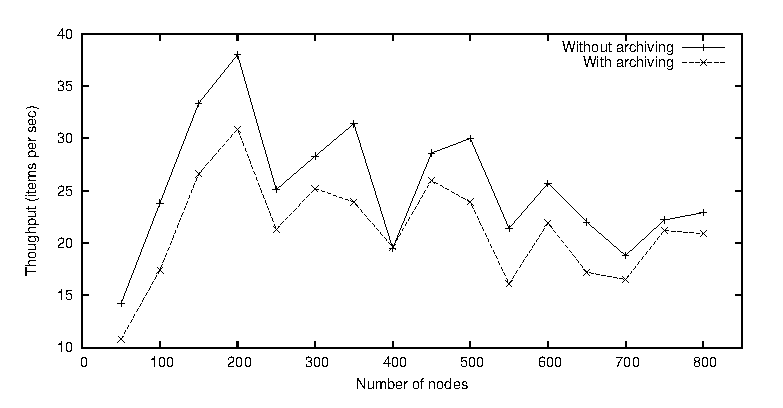
\epsfig{file=throughput.eps, width=\columnwidth}
\caption{Average throughput}
\end{center}
\end{figure}

\begin{figure}
\begin{center}
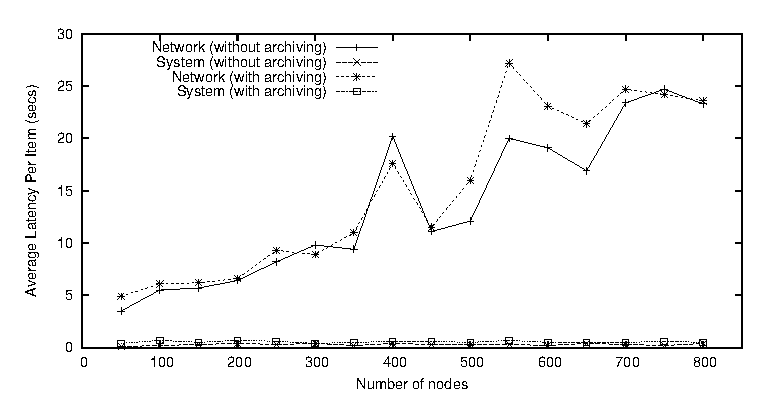
\epsfig{file=latency.eps, width=\columnwidth}
\caption{Average latencies per node}
\end{center}
\end{figure}


\begin{table*}
\begin{center}
\begin{tabular}{|l|r|r|r|r|r|r|r|r|r|r|r|r|}\hline
Num of nodes&	50&	100&	150&	200&	250&	300&	350&	400&	450&	500&	550&	600 \\ \hline\hline
Net latency per node (secs)&	9&	4&	4&	4&	8.6&	5.3&	19.1&	19.5&	14.4&	7.8&	12&	13.3 \\ \hline
Sys latency per node (secs)&	0&	0&	0&	0.3&	0.2&	0.4&	0.3&	0.1&	0.3&	0.4&	0.2&	0.7 \\ \hline
%Total Latency (secs)&	9&	4.04&	4&	4.3&	8.8&	5.8&	19.4&	19.6&	14.7&	8.2&	12.3&	14 \\ \hline
Total fetch time (secs)&	9&	5&	4&	5&	23&	9&	22&	23&	26&	14&	27&	28 \\ \hline	
Throughput (items/sec)&	5.6&	20&	37.5&	40&	10.9&	33.3&	15.9&	17.4&	17.3&	35.7&	20.4&	21.4 \\ \hline
\end{tabular}
\end{center}
\caption{Performance of Comon with no archiving}
\end{table*}


\begin{table*}
\begin{center}
\begin{tabular}{|l|r|r|r|r|r|r|r|r|r|r|r|r|}\hline
Num of nodes&	50&	100&	150&	200&	250&	300&	350&	400&	450&	500&	550&	600 \\ \hline\hline
Net latency per node (secs)&	16&	4&	4&	4&	18.9&	6&	20.6&	22&	8.4&	13&	21.8&	21.3 \\ \hline
Sys latency per node (secs)&	0.8&	1.28&	1.4&	1.8&	1.9&	1.5&	1.6&	1.3&	1.9&	1.7&	1.7&	2.2 \\ \hline
%Total Latency (secs)&	16.8&	5.28&	5.4&	5.8&	20.8&	7.5&	22.2&	23.3&	10.3&	14.7&	23.56&	23.5 \\ \hline
Total fetch time (secs)&	17&	6&	7&	7&	27&	12&	27&	30&	19&	33&	43&	43 \\ \hline
Throughput (items/sec)&	2.9&	16.7&	21.4&	28.6&	9.3&	25&	13&	13.3&	23.7&	15.2&	12.8&	14 \\ \hline
\end{tabular}
\end{center}
\caption{Performance of Comon with archiving}
\end{table*}


\section{Related Work}
\label{sec:related-work}

Given the importance of ad hoc data, it is perhaps surprising that
more tools do not exist to solve it.  Many, many tools simply assumes
that the data they manipulate is in the right format from the
beginning.  If it is not, it is up to the user to get the data in the
correct format themselves --- he or she receives little or no help
with the problem. For instance, \xml{} and relational databases expect
their inputs are already in \xml{} or standard formats such as CSV
(Comma-Separated Values).  The development of \datatype{} is
completely complementary to research on relational and semi-structured
databases as \datatype will be explicitly designed to help with the
problem of loading one of these databases with data that is not
currently in the expected format.

One might wonder why we do not choose to use tools based on regular
expressions or context-free grammars like Lex and Yacc.  First,
regular expressions and context-free grammars, while excellent
formalisms for describing programming language syntax, are not ideal
for describing the sort of ad hoc data we have discussed in this
proposal.  The main reason for this is that regular expressions and
context free grammars do not support dependency and do not support
deep semantic constraints that are important for ensuring data
integrity.  For instance, many ad hoc data sources we have studied
include ...

ASN.1~\cite{asn} and related systems~\cite{asdl} allow the user to
specify the {\em logical} in-memory representation and generate a {\em
  physical} on-disk format, but this doesn't help when given a
particular, fixed physical on-disk format.  \datatype{} helps solve
the latter problem.

More closely related work includes \erlang{}'s bit
syntax~\cite{erlang} and the \packettypes{}~\cite{sigcomm00} and
\datascript{} languages~\cite{gpce02}, all of which allow declarative
descriptions of physical data.  These projects were motivated by
parsing protocols, \textsc{TCP/IP} packets, and \java{} jar-files,
respectively.  Like \pads{}, these languages have a type-directed
approach to describing ad hoc data and permit the user to define
semantic constraints.  In contrast to our work, these systems handle
only binary data and assume the data is error-free or halt parsing if
an error is detected.  Parsing non-binary data poses additional
challenges because of the need to handle delimiter values and to
express richer termination conditions on sequences of data. These
systems also focus exclusively on the parsing/printing problem,
whereas we have leveraged the declarative nature of our data
descriptions to build additional useful tools.

Recently, a standardization effort has been started whose stated goals
are quite similar to those of the \pads{} project~\cite{dfdl}. The
description language seems to be \xml{} based, but at the moment, more
details are not available.

xduce - very similar, but for xml. Focus on static validation, not on
transformation. However, their language design of DSL pattern matching
and data constructors is parallel. no notion of error support.

%%% Local Variables: 
%%% mode: latex
%%% TeX-master: "paper"
%%% End: 


\section{Conclusions}
\label{sec:conclusion}


%{\tiny
\bibliographystyle{abbrv}
\bibliography{pads}
%}

\newpage
%\newpage
\appendix

\section{Example Data and Descriptions}
\label{app:examples}


%%% Local Variables: 
%%% mode: latex
%%% TeX-master: "semantics"
%%% End: 

\end{document}
